\documentclass[main.tex]{subfiles}


\begin{document}

\chapter{Introduction}
We all want to make good decisions. The decision
process requires understanding and prediction of systems that can
involve complex interactions fraught with uncertainty. It is, therefore,
a challenge for mathematics to come up with good practices
to guide decision makers.
This doctoral thesis contains a collection of topics that are relevant
in decision making under uncertainty, primarily motivated by
problems in the retail industry.
We present algorithms for decision making that address different
points in the decision making process.
The mathematical approach to this process consists of
five general steps, of which each chapter touch on a subset.
The steps are summarised as follows.
\begin{enumerate}\label{enum:making_decisions}
\item Objective --- statement of what the decision maker wants to achieve.
\item Model of the system --- mathematical modelling of relevant aspects
  needed to achieve the objective.
\item Data assimilation --- incorporation of available observations in
  the mathematical model.
\item Risk preference --- mathematical modelling of the decision maker's risk
  preference.
\item Optimisation --- algorithms and approximations required to
  evaluate different decisions.
\end{enumerate}

As we gain more knowledge of the system and the
impact of our decisions, the decision maker may refine their objective or
we may choose to address some of the steps differently.
This interactive process is illustrated in \Cref{fig:decision_process}.
\begin{figure}[htb]
  \centering
  \begin{tikzpicture}[node distance = 2.3cm, auto]
    % Define block styles
    \tikzstyle{block} = [rectangle, draw, fill=blue!20,
    text width=7em, text centered, rounded corners, minimum height=4em]
    \tikzstyle{line} = [draw, Latex-Latex]
    \tikzstyle{cloud} = [draw, ellipse,fill=red!20, node distance=4cm,
    minimum height=2em]
    \tikzstyle{dashline} = [draw, dashed, -{Latex[length=2.5mm]}]

    % Place nodes
    \node [block] (objective) {Define\\objective};
    \node [cloud, left of=objective, align=center] (decisionmaker) {Decision\\maker};
    \node [cloud, right of=objective] (mathematician) {Mathematician};
    \node [block, below of=objective] (modelling) {Model system};
    \node [block, below of=modelling] (data) {Data\\assimilation};
    \node [block, below of=data] (risk) {Risk preference};
    \node [block, below of=risk] (optimisation) {Formulate optimisation};
    % Draw edges
    \path [line] (objective) -- (modelling);
    \path [line] (modelling) -- (data);
    \path [line] (data) -- (risk);
    \path [line] (risk) -- (optimisation);
    \path [dashline] (decisionmaker) -- (objective);
    % \path [dashline] (decisionmaker) |- (risk);
    \path [dashline] (optimisation)  -| (decisionmaker);
    \path [dashline] (mathematician) |- (modelling);
    \path [dashline] (mathematician) |- (data);
    \path [dashline] (mathematician) |- (risk);
    \path [dashline] (mathematician) |- (optimisation);
  \end{tikzpicture}
  \caption[Decision making steps]{The steps of a mathematical approach
  to decision making. It can be an iterative approach, where the
  decision maker refines their goals after learning more about the
  system and the resulting decision impact.}\label{fig:decision_process}
\end{figure}

The mathematical decision making process, as we have defined it, is
general and can be applied to many decision problems. For a collection
of examples and arguments for a mathematical approach to decisions in
large organisations, see, for example \citet{keeney1976decisions} and
\citet{farmer2017uncertainty}.  We  use examples from the practice
of revenue management to motivate the theory and illustrate the
algorithmic approach to decision making that we present in this
thesis.

\section{Revenue management}
% The examples provided will focus on the process of setting the
% price of products; including demand modelling,
% handling of uncertainty, and optimisation algorithms.

The process of pricing products in order to control demand and
maximise revenues has been undertaken for centuries
\citep[Book~1]{smith1776inquiry}. In recent
decades, data- and model-driven approaches have become increasingly
popular in order to advise product managers and automate the process for companies.
There are several success stories from early adopters, for example in
the airline industry.
American Airlines estimated in 1992 that the introduction of revenue
management software had, over the preceding three
years, contributed \SI{500}[\$] million of additional revenue per year,
and would continue to do so in the future \citep{smith1992yield}.
In an example from Chilean retail, \citet{bitran1998coordinating}
report an expected revenue improvement of \SIrange{7}{16}{\percent} after implementing
model-driven strategies.
This range of financial impact due to implementation of pricing and revenue
management systems are further supported in other studies, see, for example, \citet[Ch.~1.2]{phillips2005pricing}.
For retailers with billions of pounds in revenues, a revenue improvement of
less than a percent can be worth millions of pounds.
In addition unsold items add up to thousands of tonnes of waste per year. So
improvements in the control of supply or demand for products would be advantageous
for both retailers and the environment.

The theory and practice of pricing and revenue management is
multidisciplinary and attracts research from a wide variety of
fields. Our focus is on different aspects of the modelling and
optimisation procedures, from a mathematical point of view.
\citet{phillips2005pricing} and \citet{ozer2012oxford} present perspectives on the
revenue management process prevalent in the social sciences.
A notable resource with more mathematical focus, which
cover both theoretical and practical
perspectives, is provided by \citet{talluri2006theory}.
Other mathematical approaches to pricing of retail products
can, for example, be found in \citet{butler2014customer}.

The objectives we focus on in this thesis are aspects of sales,
revenue, and profit targets that can be influenced by pricing
decisions.  At the core of such decisions are models connecting price
and demand of products.  In \Cref{sec:intro_model_demand} we summarise
the established approaches to demand modelling in revenue management, for
reference in later chapters.  The demand models often include
unobservable parameters that are inferred from data.  These models are
used to forecast future demand, sometimes months into the future.  The
uncertainty in future events, and in estimates of model parameters, is
described using random variables.

\subsection{Modelling demand}\label{sec:intro_model_demand}
We define demand as the quantity of a product that people are willing
to buy, per time period, at a particular price. For the purpose of our
work, demand may change over time, even if the price is constant.
For example, time-dependent aspects of demand include periodic effects, such as
seasonality and longer term trends.
In addition to pricing decisions, retailers can use advertisements and
offers to affect sales. Such demand control mechanisms often have a
more significant impact on sales than price changes in their own
right. % They are harder to forecast accurately, however, and will not
% be considered in this thesis.

The relationship between price and demand is often described in a
continuum fashion, rather than at discrete levels such as pounds or
pence. We are interested in retailers with large-scale sales and
aggregate demand models where treating the demand as a continuum gives
a reasonable approximation.
In both academia and industry, simple demand curves are often used to
model the price-demand relationship of
products. See \citet[Ch.~7.3]{talluri2006theory} or \citet{phillips2005pricing}
for a discussion of the most popular demand curves. The curves are often
chosen in order to simplify the parameter
estimation procedure, in practice, or simplify the analysis, for academic purposes.

Let $q(a)\geq 0$ denote the demand for a given product at price $a\geq 0$, holding
other aspects such as time and competitor product prices constant.
The following three demand curve families, where $q^{(1)}$ and
$q^{(2)}$ are parameters, are often used in the
revenue management literature.
\begin{align}\label{eq:demand_fun_lin}
  q(a) &= q^{(1)}-q^{(2)}a,&q^{(1)},q^{(2)}&>0,&\text{linear demand}&,\\
  q(a) &= e^{q^{(1)}-q^{(2)}a},&q^{(1)}\in\mathbb{R},q^{(2)}&>0,&\text{exponential
                                                                  demand}&\text{, and}\\
  q(a) &= q^{(1)}a^{-q^{(2)}},&q^{(1)},q^{(2)}&>0,&\text{power demand}&.\label{eq:demand_fun_pow}
\end{align}
Note that these functions should only be considered as local
approximations to demand. That is, we use these models to predict
aggregate demand responses in a neighborhood of the current
price. Care must be taken especially if one is to use the power demand
function: The demand goes to infinity as price goes to zero, and
revenues go to infinity as price goes to infinity if $q^{(2)}\in(0,1)$.
\Cref{fig:demandfun_comparison} provides a comparison of the three
demand curves which behave similarly close to the
current price, $a=1$.
\begin{figure}[htbp]
  \centering
  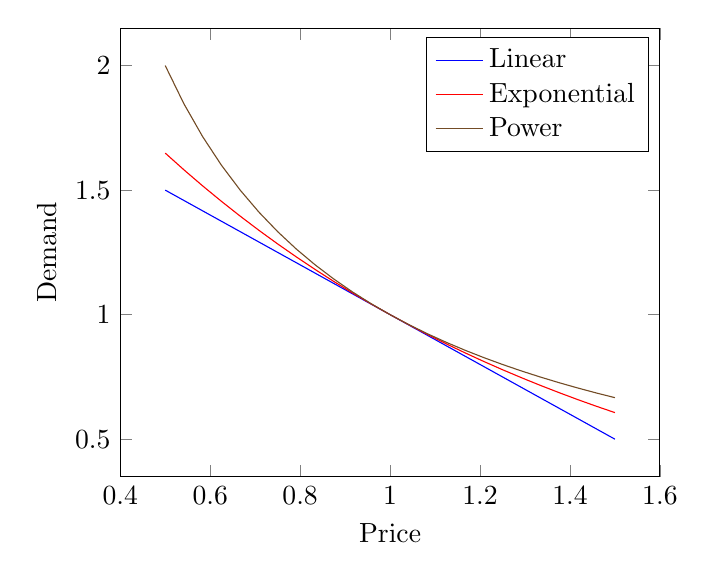
\begin{tikzpicture}[baseline]
    \begin{axis}[
      xlabel={Price},
      ylabel={Demand},
      legend cell align=left,
      ]
      \addplot+[domain=0.5:1.5, mark=none] {2-x};
      \addlegendentry{Linear}
      \addplot+[domain=0.5:1.5, mark=none] {exp(1-x)};
      \addlegendentry{Exponential}
      \addplot+[domain=0.5:1.5, mark=none] {1/x};
      \addlegendentry{Power}
    \end{axis}
  \end{tikzpicture}
  \caption[Comparison of demand curves]{Comparison of demand curves. The units of price and time
    have been re-scaled so that $q(1)=1$.}\label{fig:demandfun_comparison}
\end{figure}

In cases where we believe that the price of one product affects the
demand of another product, we introduce cross-effects on the demand
functions. For products $j=1,2,\dots,J$, denote their respective prices by
$a_j$ and their demands by $q_j(a)$, where $a=(a_1,a_2,\dots,a_J)$.
One way to extend the demand curves in~\eqref{eq:demand_fun_lin}
to~\eqref{eq:demand_fun_pow} to a multi-product case is, according to \citet{talluri2006theory},
\begin{align}
  q_j(a)&=q_{j}^{(1)}-\sum_{l=1}^Jq_{j,l}^{(2)}a_l,
  &\text{linear demand}&,\\
  q_j(a)&=\exp\left( q_{j}^{(1)}-\sum_{l=1}^Jq_{j,l}^{(2)}a_l
          \right),
  &\text{exponential demand}&\text{, and}\\
  q_j(a)&=q_j^{(1)}\prod_{l=1}^Ja_l^{-q_{j,l}^{(2)}},
  &\text{power demand}&.
\end{align}
The valid domains of the parameters vary. For example, a linear demand
model where we believe that increasing the price of product $l$ has a
positive effect on the demand of product $j$ constrains
$q_{j,l}^{(2)}$ to be negative. \Cref{fig:demand_exponential_two}
provides an example of demand for a given product when varying
its price and the price of one competing product, using the exponential demand function.
\begin{figure}[htbp]
  \centering
  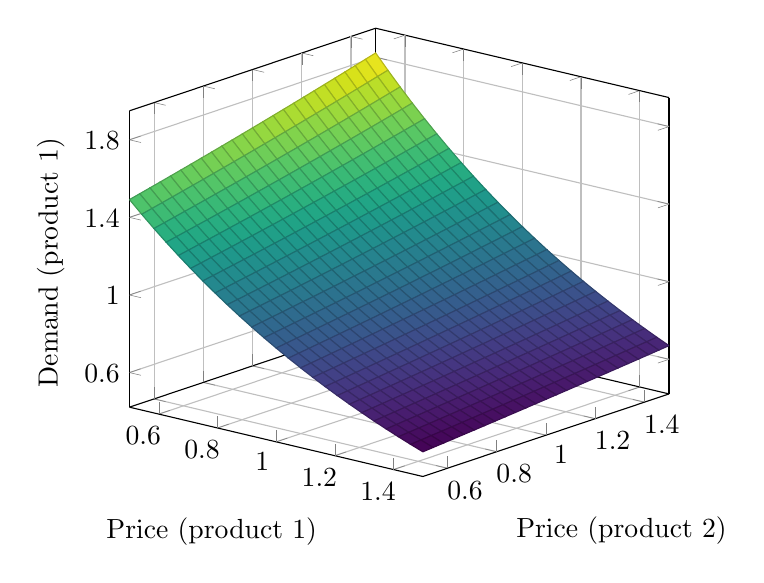
\begin{tikzpicture}
    \begin{axis}[
      domain=0.5:1.5,
      xlabel={Price (product 1)},
      ylabel={Price (product 2)},
      zlabel={Demand (product 1)},
      view={40}{20},
      colormap/viridis,
      xmajorgrids={true}, ymajorgrids={true}, zmajorgrids={true},
      xtick={0.6,0.8,1,1.2,1.4},
      ytick={0.6,0.8,1,1.2,1.4},
      ztick={0.6,1,1.4,1.8},
      ]
      \addplot3[surf]
      {exp(1-0.2-1*x+0.2*y)};
    \end{axis}
  \end{tikzpicture}
  \caption[Exponential demand function]{Exponential demand function for product $1$, with one
    competing product $j=2$.
    Units are rescaled so that $q_1(\vecbracks{1,1})=1$.
  }\label{fig:demand_exponential_two}
\end{figure}

\begin{remark}
  Note that both the exponential
  and power demand functions are unbounded: The demand of a product
  $j$ goes to infinity if we take the price of some product $l\neq j$
  to infinity, provided $q_{j,l}^{(2)}<0$. One way that practitioners
  address this issue is to define hard constraints on the prices, such as
  keeping the new price within \SI{20}{\percent} of the current price.
  In \Cref{ch:onestage} we address this issue in a different way by
  providing an alternative model for cross-effects.
\end{remark}

\subsection{Forecasting and uncertainty}
Demand models, such as those presented above, have parameters that are
product specific, and which must be estimated before forecasts of
demand can be made.
As multi-month forecasts may be required by the retailer, better
approximations to future demand are perhaps possible with
time-dependencies in the parameters.
This estimation procedure is often guided by
historic sales data collected by the retailer, using data assimilation
techniques \citep{law2015data,riseth2017operator} or time series analysis
\citep{chatfield2004analysis}.
% \todo[inline]{Provide example of time-dependent modelling? 1)
%   Sinusoidal model, 2) Model based on neighbouring values, linear
%   combination of previous time periods (in a periodic domain,
%   i.e. both the most recent, and in previous years/months)}

The models used to forecast future demand at particular prices carry
a range of errors and uncertainty. First, estimates of parameter
values are affected by uncertainty and numerical errors. Second, the model form may be
inappropriate. Third, exogenous events impact demand outcomes in a more general
way.
% These sources of uncertainty are all epistemic, meaning
% that one can reduce them by refining models and gathering more
% data.
% Fourth, uncertainties that are aleatory, which refers to inherent
% uncertainty in a system that cannot be reduced. See
% \cite{der2009aleatory} for a discussion on aleatory and epistemic
% uncertainty.
% One may argue the philosophical point whether uncertainty that is
% aleatory exists, however, it does not change our approach to modelling
% the uncertainty in our forecasts.
A forecast is in essence an extrapolation of an evaluated model to a
region of the input domain not yet experienced. We may still have an
idea of what form the uncertainty this extrapolation takes, which
we model in terms of random variables.

For example, consider a product for which we forecast the sales for
two consecutive periods using the exponential demand model,
\begin{equation}
  q(t,a) =
  e^{q^{(1)}(t)-q^{(2)}(t)a},\qquad t=1,2.
\end{equation}
To quantify the uncertainty in our model parameters, we associate
with each of $q^{(1)}(t)$, $q^{(2)}(t)$ a probability distribution, not
necessarily independent.
Let $W(t,a)$ denote a random field that expresses the uncertainty
associated with exogenous events and extrapolation outside the
observed price region.
We forecast the demand in period $t$ to be $Q(t,a)=q(t,a)W(t,a)$, and
the total forecasted demand is thus the random variable $Q(1,a_1) +
Q(2,a_2)$, where $a_t$ denotes the planned price in period $t$.
Illustrations of the distributions of objectives and example models of
$W(t,a)$ are provided in
\Cref{ch:onestage,ch:discrete_control,ch:cts_control}.

% \section{Decisions via optimisation}\label{sec:intro_decisions_through_optim}
% Optimisation is central to our approach to decision making, and will
% be integral to all the chapters in the thesis.
% We will cover optimisation in the context of multiple objectives,
% one-stage decision problems, sequential decision problems, parameter
% estimation, and in algorithm design.
% All the problems we consider will eventually confirm to a general
% form. For some decision set $\mathcal{X}$, and a mapping
% $\mathcal{F}:\mathcal{X}\to\mathbb{R}$ that is bounded below, we
% formulate the decision problem as finding a solution to
% \begin{equation}
%   \min_{x\in\mathcal{X}}\mathcal{F}(x).
% \end{equation}
% The set $\mathcal{X}$ may be a subset of a finite or
% infinite-dimensional space. Whenever the problem needs to be solved by
% a numerical approach, we discretise the set and consider
% finite-dimensional approximations $X\subset\mathbb{R}^n$, $f:X\to\mathbb{R}$ to
% $\mathcal{X}$ and $\mathcal{F}$ respectively.
% The set $X$ can be defined either implicitly, or explicitly, in the
% form of a collection of equality and inequality constraints,
% \begin{equation}
%   X = \{x\in\mathbb{R}^n\mid c_i(x)=0, c_k(x)\geq 0, \text{ for }
%   i\in\mathcal{I},\;j\in\mathcal{J}\}.
% \end{equation}
% \todo[inline]{Minimise vs maximise}
% \todo[inline]{Local minima}
% The theory of optimisation of functions on $\mathbb{R}^n$, and
% algorithms to approximate solutions to such problems, are well covered
% by~\citet{nocedal2006numerical}. We will often refer to this book in
% the context of optimisation.

% \section{Preliminary probability and random variables}\label{sec:intro_prob_rvs}
% \todo[inline]{Do we need this?}

\section{Outline of thesis}
We present the chapters in this thesis by connecting them to the
steps for making decisions that are listed
on Page~\pageref{enum:making_decisions} and in \Cref{fig:decision_process}.
In \Cref{ch:onestage} we focus on the general discussion of the
``objective'', ``risk preferences'', and ``optimisation''.
\Cref{ch:onestage} contains much of the background material on formulating
optimisation problems and can be considered an extension to this
introductory chapter. We introduce one-stage optimisation problems with
random outcomes and multi-objective optimisation.
A comparison of risk preference methods shows that simple and more complicated
methods can yield very similar decisions. Therefore, the choice of
method should focus on implementational and computational aspects
rather than theoretical arguments.
In \Cref{ch:discrete_control} and
\Cref{ch:cts_control} we present  aspects of the steps ``model of the system'', ``risk
preferences'', and ``optimisation'' for sequential decision problems
in discrete and continuous time.
\Cref{ch:discrete_control,ch:cts_control} provide examples of
how simplified formulations, that ignore the randomness, result in
marginalised outcomes that are practically equal to the values from
decisions based on the original formulation. A further investigation
of the distribution of outcomes shows that the simplified formulations
result in the best outcomes for half of the realisations of the
underlying random variables. In the remaining realisations, they
result in much worse outcomes, which we interpret as an algorithmic
decision that has impacted the modelled risk-attitude.

The first chapters are closely linked to the application of pricing
in retail, whilst the penultimate chapter has a mathematical focus
independent of particular applications.
% \Cref{ch:koopestim} looks at a novel way to handle the Data
% assimilation step.
\Cref{ch:objaccel} presents a new
algorithm to improve the optimisation step. The algorithm can be
be combined with existing algorithms and we show, with several
numerical experiments, that it reduces the computational cost of
finding a solution with a prescribed accuracy.
The general implications the findings in this thesis are covered in
\Cref{ch:conclusion}.

\section{Statement of originality}
\subfile{originality}

\biblio{} % Bibliography when standalone
\end{document}

%%% Local Variables:
%%% mode: latex
%%% TeX-master: t
%%% TeX-command-extra-options: "--shell-escape"
%%% End:
